Even if the number of parents k is smallish, fill any CPT requires $O(2^k)$ numbers and it grows exponentially with number of parents. Instead, if we assume a 
continuous-valued parent or child, CPT becomes \textbf{infinite}\footnote{One of the nicest thing of Bayesian network is the capability to combine together
different types of variables, sush as descrete, continuos, deterministic, not-deterministic and so on.}. Usually, a solution to solve these types of
problem consists of \textbf{canonical distributions}. \vspace{3.5pt}

The simplest case is provided by \textbf{deterministic nodes}:
\begin{center}
    $X = f(Parents(X))$
\end{center}
A deterministic node has its values specified exactly by the values of its parents, with no uncertainty.
\begin{example}
    i.e. Logical relationship, so there is no stochasticity. \vspace{3.5pt}

    The relationship between the parent nodes $(Canadian, US, Mexico)$ and the child node $(NorthAmerican)$ is simply that the child is the disjunction, or the logical OR,
    of the parents. \vspace{3.5pt}

    \begin{center}
        \begin{tabular}{|c|c|c|c|}
            \hline
            \bf Canadian & \bf US & \bf Mexico & \bf NorthAmerican  \\
            \hline
            F & F & F & F \\
            T & F & F & T \\
            F & T & F & T \\
            F & F & T & T \\
            T & T & F & T \\
            T & F & T & T \\
            F & T & T & T \\
            T & T & T & T \\
            \hline
        \end{tabular}
    \end{center} \vspace{7pt}

    i.e. Numerical relationship. \vspace{3.5pt}
    
    If the parent nodes are a lake's inflows $(Rivers, Runoff, Precipitation)$ and the outflows $(Rivers, Evaporation, Seepage)$ and the child node is the
    change in the water level of the lake, then the value of the child is the sum of the inflow parents minus the sum of the outflow parents. \vspace{3.5pt}

    \begin{center}
        $\frac{Level}{t}=inflow+precipitation-outflow-evaporation$
    \end{center}
\end{example}

Another interesting example is the \textbf{Noisy-OR distribution}, which is very useful representation. Now, we will describe an example to understand the intuition
of Noisy-OR distribution given a medical domain.
\begin{example}
    i.e. Medical representation. \vspace{7pt}

    \begin{center}
        \begin{tabular}{|c|c|c|c|c|}
            \hline
            \bf Cold & \bf Flu & \bf Malaria & \bf P(Fever) & \bf P($\mathbf{\neg Fever}$) \\
            \hline
            F & F & F & 0.0 & \dots \\
            \hline
        \end{tabular}
    \end{center} \vspace{7pt}

    Imagine that you are looking to the symptom, which is the $(Fever)$, and the symptom can be caused by different deseases, such as $(Cold, Flu, Malaria)$.
    However, the network is defined by three different causes parent of the same effect. \vspace{3.5pt}
    
    As we can suppose, it is very common in medical domain to diagnose the cause given the symptom, $(Fever)$. Furthermore, as written before,
    the size of this representation is exponential, it requires $2^3$ parameters, and it encreases with the number of the parents. \vspace{3.5pt}

    We can make some simplified assumptions, that let us to reduce the size of the representation from exponential to linear with the number of parents. For instance,
    $Malaria$ in the $90\%$ of the cases will cause $Fever$, in the last $10\%$ fails to cause $Fever$. This is called the \textbf{failure probability}. \vspace{3.5pt}

    The second row of the table shows what we are talking about: we got $Malaria$ but not the other symptoms and the probability of not having $(Fever)$ is 0.1. \vspace{3.5pt}

    The main idea about failure probabilities is that each of them is independent from other failure probabilities. So, if we got $(Flu, Malaria)$ but not $(Cold)$ then the 
    failure probability will be $0.1 \times 0.2=0.2$, mixed failure probabilities are solved by the product of each single failure probability.
\end{example}
Generally, Noisy-OR distributions by failure probabilities let to reduce the size of representations from exponential to linear, the initial table has the same number of 
parameters such as the number of parents present. The failure probabilities let us to solve every question about the domain analyzed.
Despite Noisy-OR distribution is a powerful tool, this works only if all the causes are already listed there and all the variables
are Boolean.
\begin{definition}
    \textbf{Noisy-OR distributions} model multiple causes for the same effect if and only if:
    \begin{itemize}
        \renewcommand{\labelitemi}{-}
        \item Parents $U_1, \dots, U_k$ include all causes\footnote{If missing, we can add the \textbf{leak node}.}.
        \item Each failure probability is independent from other failure probabilities.
    \end{itemize} \vspace{7pt}

    \begin{center}
        $P(X|U_1 \dots U_k, \neg U_{j+1} \dots \neg U_k) = 1 - \prod_{i=1}^{j} q_i$
    \end{center} \vspace{3.5pt}

    Where $q_i$ stands for \textbf{failure probability} of \textbf{i cause}.
\end{definition}
\textbf{Hybrid networks} \vspace{3.5pt}

Many real-world problems involve continuos quantities, such as money, temperature, height and mass; in fact, much of statistics deals with random variables
whose domains are continuos. By definition, continuos variables have an infinite number of possible values, so it is impossible to specify conditional
probabilities for each value. There are many different ways to handle continuos variables:
\begin{itemize}
    \renewcommand{\labelitemi}{-}
    \item \textbf{Discretization}: dividing up the possible values into a set of intervals. Discretization is sometimes an adequate solution, but often results in 
    large errors and the CPTs could be quite huge.
    \item \textbf{Finitely parameterized canonical families}: the most common way is to define standard families of probability density functions that are specified
    by a finite number of parameters. 
\end{itemize}
A network with both discrete and continuos variables is called \textbf{hybrid Bayesian network}. To design a hybrid network, we have to specify two new kinds of 
distributions:
\begin{itemize}
    \renewcommand{\labelitemi}{-}
    \item the conditional distribution for a continuos variable given discrete or continuos parents;
    \item the conditional distribution for a discrete variable given continuos parents.
\end{itemize}
Let's set a new example for better understanding.
\begin{example}
    i.e. Harvest hybrid network. \vspace{3.5pt}

    \begin{center}
        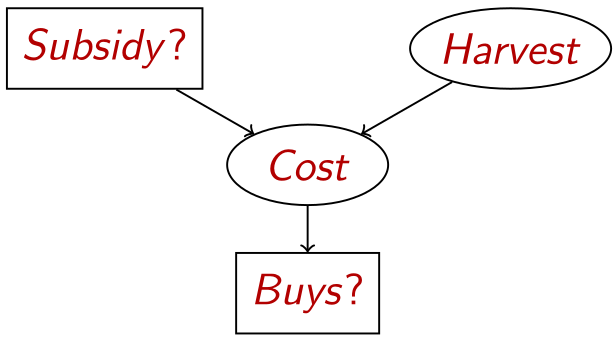
\includegraphics[width=0.4\textwidth]{img/img11.png}
    \end{center} \vspace{3.5pt}
    Consider the network shown previously, in which a customer buys some fruit depending on its cost, which depends in turn on the size of the harvest and from the 
    government's subsidy. The variable $(Cost)$ is continuos and has continuos and descrete parents $(Harvest, Subsidy)$, the variable $(Buys)$ is descrete and it has
    a continuos parent. \vspace{3.5pt}

    One standard way to represent the first type of relationship is the \textbf{Linear Gaussian Model}, where the distribution of $Cost$ is the Gaussian distribution 
    with fixed \textbf{variance} and variable \textbf{mean}. The mean depends on the value of the \textbf{continuos parent} $(Harvest)$, and it can be represented
    as a linear function of $(Harvest)$. Moreover, the parameters $(a, b)$ of the mean change based on presence or absence of $(Subsidy)$. \vspace{3.5pt}

    \begin{center}
        $P(Cost = c|Harvest = h, Subsidy ?= true) =$
        $N(a_th+b_t, \sigma_t)(c) = \frac{1}{\sigma_t\sqrt{2\pi}}e^{-\frac{1}{2}(\frac{c - (a_th+b_t)}{\sigma_t})^2}$
    \end{center} \vspace{7pt}
    Before moving on, we focus on some aspects of the equation:
    \begin{itemize}
        \renewcommand{\labelitemi}{-}
        \item $(a_*h+b_*)$ defines the mean of the distribution, if $h$ changes also the mean will change\footnote{The star $(*)$ symbols stand for the enumeration of $(Subsidy)$.}.
        \item $(\sigma_*)$ is the standard deviation, which is fixed, never change.
        \item Presence or abscence of $(Subsidy)$ determines the choice of $(a, b)$ parameters, but it hasn't any influence on $(Harvest)$ behavior, again,
        if it encreased the cost could decrease and vice versa.
    \end{itemize} \vspace{7pt}

    Now we turn to the distributions for descrete variables with continuos parents. We now consider the $Buys$ node. It seems reasonable to assume that the customer will buy if the cost is low 
    and will not buy if it is high and the probability of buying varies smoothly in some intermediate region. In other words, the conditional distribution is like a soft threshold function. \vspace{3.5pt}

    There are two ways to make soft threshold, as:
    \begin{itemize}
        \renewcommand{\labelitemi}{-}
        \item \textbf{Probit distribution}, uses the integral of the standard normal distribution to compute a threshold.
        \item \textbf{Sigmoid distribution}, uses the \textit{logistic function} to produce a soft threshold\footnote{The sigmoid or logit distribution is widely used in neural networks, more than the probit one.}.
        \begin{center}
            $P(Buys? = true | Cost = c) = \frac{1}{1+e^{(-2^{(\frac{-c+\mu}{\sigma})})}}$
        \end{center}
    \end{itemize}
\end{example}